\documentclass[12pt,letterpaper]{article}
\usepackage{preamble}

\newcommand\course{Linear Control Theory}
\newcommand\hwnumber{5}
\newcommand\userID{Daniil Manakovskiy}
\newcommand\userGroup{BS18-02}

\begin{document}
Variant: A

Email: d.manakovskiy@innopolis.university

The given dynamics:
\begin{equation}
    \label{given:1}
    (M + m)\ddot x - ml \ddot \theta \cos(\theta) + ml \dot\theta^2 \sin(\theta) = F
\end{equation}

\begin{equation}
    \label{given:2}
    - \ddot x \cos(\theta) + l \ddot\theta - g\sin(\theta) = 0
\end{equation}

where $M = 7.5, m = 4.4, l = 1.2, g = 9.81$

The system can be written in a state space form:
\begin{equation*}
    \begin{cases}
    \dot z = f(z) +g(z)u \\
    y = h(z) = 
        \begin{bmatrix}
            x & \theta 
        \end{bmatrix}  \T
    \end{cases}
\end{equation*} 

where $z = 
    \begin{bmatrix}
        x & \theta & \dot x & \dot \theta 
    \end{bmatrix}  \T$
    
The system can also be linearized around $\bar z = \begin{bmatrix}
            0 & 0 
            & 0 
            & 0
        \end{bmatrix} \T$
as was done in \href{https://github.com/WinnerOK/LinearControl_assignments/tree/assignment_dev/HomeWork4}{Homework4}:
\begin{equation*}
    \begin{cases}
        \delta \dot z = A \delta z + B \delta u \\
        \delta y = C \delta z
    \end{cases}
\end{equation*}

\begin{equation*}
    \begin{cases}
        \delta \dot z =     
        \begin{bmatrix}
            0 & 0                   & 1 & 0\\ 
            0 & 0                   & 0 & 1\\ 
            0 & \frac{gm}{M}        & 0 & 0\\[10pt] 
            0 & \frac{g(m+M)}{Ml}   & 0 & 0
        \end{bmatrix}
        \delta z
        +
        \begin{bmatrix}
            0\\ 
            0\\ 
            \dfrac{1}{M}\\[10pt] 
            \dfrac{1}{Ml}
        \end{bmatrix}
        \delta u \\
        \delta y = 
            \begin{bmatrix}
            1 & 0 & 0 & 0 \\
            0 & 1 & 0 & 0
            \end{bmatrix}
            \delta z
    \end{cases}
\end{equation*}

\begin{equation*}
    \begin{cases}
        \delta \dot z =     
        \begin{bmatrix}
            0 & 0                   & 1 & 0\\ 
            0 & 0                   & 0 & 1\\ 
            0 & 5.7552              & 0 & 0\\
            0 & 12.971              & 0 & 0
        \end{bmatrix}
        \delta z
        +
        \begin{bmatrix}
            0\\ 
            0\\ 
            0.133\\
            0.111
        \end{bmatrix}
        \delta u \\
        \delta y = 
            \begin{bmatrix}
            1 & 0 & 0 & 0 \\
            0 & 1 & 0 & 0
            \end{bmatrix}
            \delta z
    \end{cases}
\end{equation*}


\section*{Task A. Determining observability.}
\label{Q:A}
    To verify that it is possible to design an observer for linearized system, we have to construct observability matrix $O^{np \times n}$, where $n=\dim(x)=4, p=\dim(y)=2$:
    \begin{equation*}
        O =
            \begin{bmatrix}
            C       \\
            CA      \\
            CA^2    \\
            CA^3
            \end{bmatrix}
    \end{equation*}
    if $rank(O) = n = 4$, then it is possible to design a controller. Code for finding $O$ is present at listing \ref{code:observability_matrix}.
     
    \lstinputlisting[language=Python,caption={Finding observability matrix $O$}, label={code:observability_matrix}, linerange={1-32}]{code/observability.py}
     
    Let us see the matrix itself and its rank:
    \begin{verbatim}
>>> print(f"Observability matrix:\n{O}\n\nShape:{O.shape}\nrank: {matrix_rank(O)}")

Observability matrix:
[[ 1.      0.      0.      0.    ]
 [ 0.      1.      0.      0.    ]
 [ 0.      0.      1.      0.    ]
 [ 0.      0.      0.      1.    ]
 [ 0.      5.7552  0.      0.    ]
 [ 0.     12.971   0.      0.    ]
 [ 0.      0.      0.      5.7552]
 [ 0.      0.      0.     12.971 ]]

Shape:(8, 4)
rank: 4
    \end{verbatim}
    
    As we see, the observability matrix has dimensions $8 \times 4$ and rank $4$, so it is possible to design an observer.

\section*{Task B. Exploring openloop observer.}
\label{Q:B}
    Openloop observer is just a simulation of a system dynamics. In case we know initial conditions, we will get 100\% observation, otherwise nothing is guaranteed. Listing \ref{code:openloop_stable_error} considers system stabilized using LQR, to observe unstable system, replace line 39 to 
    \begin{verbatim}return np.array([1])\end{verbatim}
    For the code I decided to change $x$ and $\theta$ in initial conditions since in real life we almost never know them.
    
    % \lstinputlisting[language=Python,caption={Open-loop observation error for unstable system}, label={code:openloop_unstable_error}]{code/openloop_unstable.py}

    \lstinputlisting[language=Python,caption={Open-loop observation error for stable system}, label={code:openloop_stable_error}]{code/openloop_stable.py}
    
    Figure \ref{fig:openloop_error} compares error dynamics on unstable and stabilized system. As we can see at figure \ref{fig:openloop_unstable_error} an error dynamics in unstable, since initial conditions differ and the system itself is unstable. Figure \ref{fig:openloop_stable_error} shows stable error dynamics, because LQR eventually converges on every initial conditions, so at some moment we will see both: real state and estimation to be equal to 0, which is not really interesting to us.
    
    \begin{figure}[htb]
        \begin{subfigure}{.5\textwidth}
            \centering
            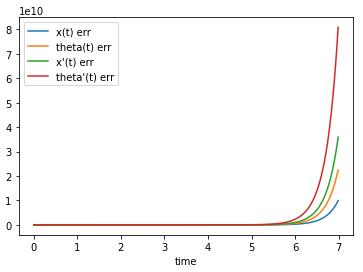
\includegraphics[width=1\linewidth]{images/openloop/unstable.jpg}
            \caption{Unstable system}
            \label{fig:openloop_unstable_error}
        \end{subfigure}
        \begin{subfigure}{.5\textwidth}
          \centering
          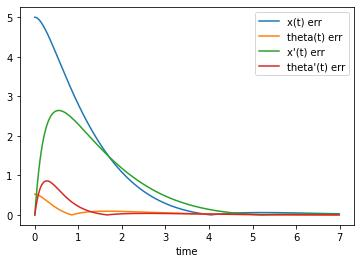
\includegraphics[width=1\linewidth]{images/openloop/stabilized.jpg}
          \caption{Stabilized system}
        \label{fig:openloop_stable_error}
        \end{subfigure}
    \caption{Open-loop observation error}
    \label{fig:openloop_error}
    \end{figure}

\section*{Task C. Designing Luenberger observer.}
\label{Q:C}
    According to \href{https://www.mathworks.com/help/physmod/sps/ref/luenbergerobserver.html}{MathWorks} Luenberger observer has the following form:
    \begin{equation*}
        \hat x(t+1) = A \hat x(t) + Bu(t) + L( y(t) - \hat y(t)
    \end{equation*}
    where $A - LC \prec 0$
    
    \subsection*{LQR solution}
        We can find matrix $L$ by solving dual problem using LQR:
        \begin{equation*}
            A - LC \prec 0
        \end{equation*}
        
        \begin{equation*}
            (A-LC)\T \prec 0
        \end{equation*}
        
        \begin{equation*}
            A\T-C\T L\T \prec 0
        \end{equation*}
        
        \begin{equation*}
            L\T = \text{lqr}(A\T, C\T, Q, R)
        \end{equation*}
        
        \begin{equation*}
             L = \text{lqr}(A\T, C\T, Q, R)\T
        \end{equation*}
        Code equivalent is at listing \ref{code:luenberg_lqr_obs}.
        
        \lstinputlisting[language=Python,caption={Calculating matrix L for Luenberg observer via LQR}, label={code:luenberg_lqr_obs}, linerange={1-14}]{code/luenberg.py}
    \subsection*{Pole Placement}
        Having derived dual problem:
        \begin{equation*}
            A\T-C\T L\T \prec 0
        \end{equation*}
        We can use pole placement to obtain L:
        \begin{equation*}
            L\T = place\_poles(A\T, C\T, desired\_poles).gain\_matrix
        \end{equation*}
        
        \begin{equation*}
            L = place\_poles(A\T, C\T, desired\_poles).gain\_matrix\T
        \end{equation*}
        
        Code equivalent is at listing \ref{code:luenberg_pole_obs}.
        \lstinputlisting[language=Python,caption={Calculating matrix L for Luenberg observer via LQR}, label={code:luenberg_pole_obs}, linerange={16-19}]{code/luenberg.py}
        
    \subsection*{Implementation}
        In order not to implement custom ODE solver, I decided to use a trick proposed by students of 4th group:
        to use $odeint$ on local timeline comprised of 2 neighbour timestamps.
        
        Brief explanation of a code:
        \begin{itemize}
            \item Function \textbf{real} is responsible to calculate real value of $x$ for given time $t$ and input $u$.
            \item \textbf{luenberg} function calculates Luenbeg observation at time $t$ with input $u$ and sensor measurement $y$.
            \item Then we setup initial values. Initial values for real system and observer are different since observer almost never know real initial ones.
            \item finally, in a loop we calculate observation and real values step-by-step.
        \end{itemize}
        
        Source code is at listing \ref{code:luenberg}.
        \lstinputlisting[language=Python,caption={Calculating Luenberg observer}, label={code:luenberg}, linerange={22-84}]{code/luenberg.py}
        
        As a result on uncotrolled system we see observation error going to infinity (figure \ref{fig:luenberg_uncontrolled}). The reason for it is that the system is unstable, therefore goes to infinity, so even small approximation error also goes to infinity. The result will be better when we stabilize the system.
        
        \begin{figure}[htb]
        \begin{subfigure}{.5\textwidth}
            \centering
            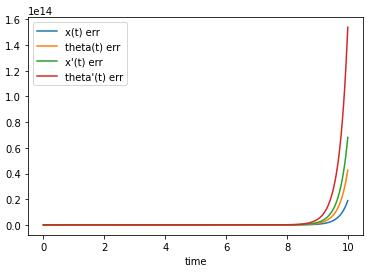
\includegraphics[width=1\linewidth]{images/luenberg/L_pole_uncontrolled.jpg}
            \caption{Pole placement}
            \label{fig:luenberg_uncontrolled_pole}
        \end{subfigure}
        \begin{subfigure}{.5\textwidth}
          \centering
          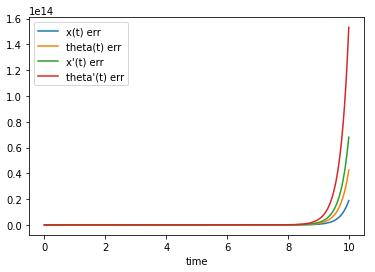
\includegraphics[width=1\linewidth]{images/luenberg/L_lqr_uncontrolled.jpg}
          \caption{LQR}
        \label{fig:luenberg_uncontrolled_lqr}
        \end{subfigure}
    \caption{Luenberg observer on uncontrolled system}
    \label{fig:luenberg_uncontrolled}
    \end{figure}

\newpage
\section*{Task D. Designing feedback controller.}
\label{Q:D}
    This task was done at \href{https://github.com/WinnerOK/LinearControl_assignments/tree/assignment_dev/HomeWork4}{HomeWork4}.
    
    Stabilization is present in code at 
    \lstinputlisting[language=Python,caption={Stabilizer}, label={code:stabilizer}, linerange={17-17, 60-60, 62-62, 67-68}]{code/luenberg.py}

\section*{Task E. Simulate system with Luenberg observer and controller.}
\label{Q:E}
    The source code is the same as shown at listing \ref{code:luenberg}. The results are present at figure \ref{fig:luenberg_controlled}. As we can see error converges to 0 relatively fast. Convergence at LQR is not that smooth because $R$ matrix dominates over $Q$.
    
    \begin{figure}[htb]
        \begin{subfigure}{.5\textwidth}
            \centering
            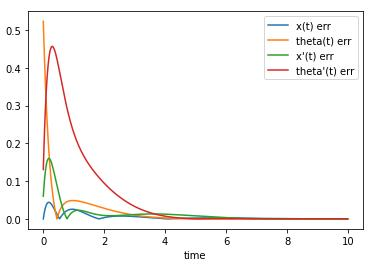
\includegraphics[width=1\linewidth]{images/luenberg/L_pole_controlled.jpg}
            \caption{Pole placement}
            \label{fig:luenberg_uncontrolled_pole}
        \end{subfigure}
        \begin{subfigure}{.5\textwidth}
          \centering
          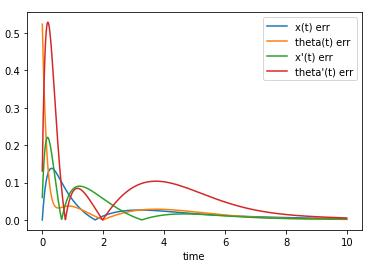
\includegraphics[width=1\linewidth]{images/luenberg/L_lqr_controlled.jpg}
          \caption{LQR}
        \label{fig:luenberg_uncontrolled_lqr}
        \end{subfigure}
    \caption{Luenberg observer on controlled system}
    \label{fig:luenberg_controlled}
    \end{figure}

\section*{Task F. Add white noise to the output.}
\label{Q:F}
    After adding noise generated by \textit{numpy.random.randn} and multiplying it by scale constant 0.5 we obtain the result presented at figure \ref{fig:output_noise_05}. Observer output becomes noise thus observation error also changes rapidly.

    
    \begin{figure}[htb]
        \begin{subfigure}{.5\textwidth}
            \centering
        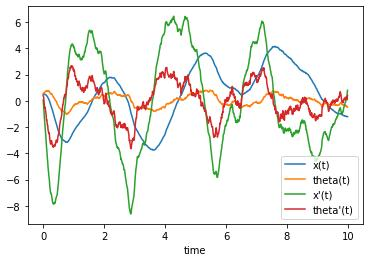
\includegraphics[width=1\linewidth]{images/filter/output_noise_05.jpg}
        \caption{Observer output}
        \label{fig:output_noise_05_obs}
        \end{subfigure}
        \begin{subfigure}{.5\textwidth}
          \centering
          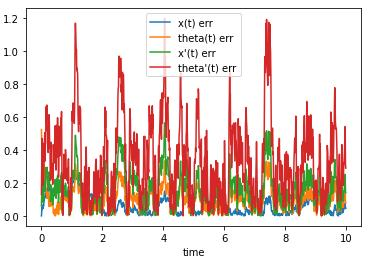
\includegraphics[width=1\linewidth]{images/filter/output_noise_05_err.jpg}
          \caption{Observation error}
        \label{fig:output_noise_05_err}
        \end{subfigure}
    \caption{System behaviour with output noise scaled by 0.5}
    \label{fig:output_noise_05}
    \end{figure}

\section*{Task G. Add white noise to the dynamics.}
\label{Q:G}
    As you see, previously I have widely used odeint as DE solb a DE solver, but I experienced problems with it, because it uses 'Adams/BDF method with automatic stiffness detection and switching.' according to \href{https://docs.scipy.org/doc/scipy/reference/generated/scipy.integrate.LSODA.html#scipy-integrate-lsoda}{docs.scipy.org}. I do not why, but it causes odeint to work very slow on noise data and produce some internal errors. After this I decided to switch to Runge-Kutta solver. The code is available under 'Kalman filter' section of the source code. As a result at figure \ref{fig:noise_dynamics} we can see noisy states.
    
    \begin{figure}[htb]
        \centering
        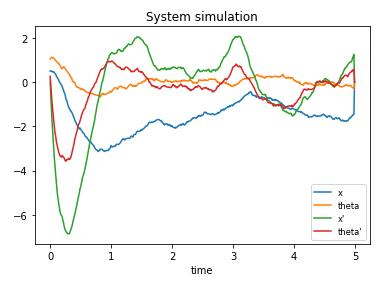
\includegraphics[width=0.5\linewidth]{images/filter/noisy_dynamics.jpg}
        \caption{Noisy dynamics.}
        \label{fig:noise_dynamics}
    \end{figure}

\section*{Task H. Implement Kalman Filter.}
\label{Q:H}
    Theory on Kalman filter is taken from \href{https://en.wikipedia.org/wiki/Kalman_filter}{Wikipedia} and Lab 11. The source code is shown at listing \ref{code:kalman}
    
    \lstinputlisting[language=Python,caption={Kalman Filter implementation.}, label={code:kalman}]{code/kalman.py}

\section*{Task I. Kalman Filter correctness.}
\label{Q:I}
    % Behaviour of Kalman filter on the given dynamics is shown at figure \ref{fig:output_noise_0005_filtered}. You can notice that noise was down-scaled to $0.005$ since at higher magnitude filter resulted in numerical instability. After some rapid changes predictions stabilize with final precision ~0.05. \nameref{fig:kalman_uncontrolled} is similar to the situation at \nameref{fig:luenberg_uncontrolled}: small observation error tends to infinity when the system is unstable. If to consider all states, prediction error behaves similarly (fig. \ref{fig:kalman_prediction_error}).
    
    Initially I had an error in the usage of the filter. Having fixed that I understood that now I have another problem: if I pass $u$ to the KF predict function, the output becomes numerically unstable. Although if time\_step is small enough, result becomes much better (see figure \ref{fig:output_noise_0005_filtered}). \nameref{fig:kalman_uncontrolled} is similar to the situation at \nameref{fig:luenberg_uncontrolled}: small observation error tends to infinity when the system is unstable. As well error on stabilized system eventually converges to 0 (fig. \ref{fig:kalman_prediction_error}).
    
    
    \begin{figure}[htb]
    \centering
        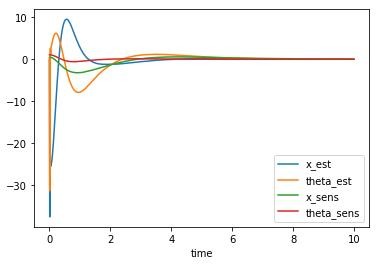
\includegraphics[width=0.5\linewidth]{images/filter/kalman.jpg}
    \caption{Kalman filter with 0 input}
    \label{fig:output_noise_0005_filtered}
    \end{figure}
    
    \begin{figure}[htb]
        \centering
        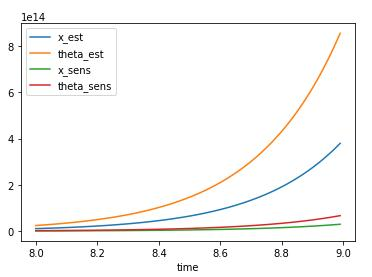
\includegraphics[width=0.5\linewidth]{images/filter/kalman_uncontrolled.jpg}
        \caption{Kalman predictions on uncontrolled system.}
        \label{fig:kalman_uncontrolled}
    \end{figure}
    
    \begin{figure}[htb]
        \centering
        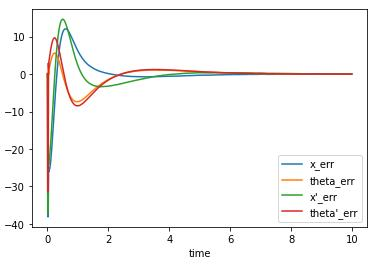
\includegraphics[width=0.5\linewidth]{images/filter/kalman_prediction_error.jpg}
        \caption{Kalman prediction error on controlled system.}
        \label{fig:kalman_prediction_error}
    \end{figure}
    
\section*{Task J. LQG controller.}
\label{Q:J}
    LQG is a combination of a LQR and LQE (Kalman filter). Since both LQR and LQE - the best controller and estimator, their combination also guarantees stability, but there is a catch: sometimes controller designed using state-space tools are sensitive to errors in the knowledge of the system dynamics. My controller diverges, I think this happens due to relatively big errors at the beginning of observation (fig \ref{fig:kalman_prediction_error}) and the controller does not recover from such mistakes. It seems to me, that the problem is in the description of matrices Q and R for Kalman Filter (matrices stating for noise covariances).
\end{document}
